\documentclass[a4paper]{article}

\usepackage[english]{babel}
\usepackage[utf8]{inputenc}
\usepackage{amsmath}
\usepackage{graphicx}
%\usepackage[colorinlistoftodos]{todonotes}

\title{Elaborazione di dati tridimensionali: homework 2}

\author{Alberto Cenzato 1134707}

\date{\today}

\begin{document}
\maketitle

\begin{abstract}
Scopo di questo secondo homework era di familiarizzare con la libreria PCL. Sono stati svolti quattro esercizi di complessità crescente per approfondire diverse funzionalità di PCL: lettura di point cloud da file, lettura e visualizzazione dei valori contenuti nella point cloud, downsampling, calcolo di normali, keypoint e descrittori, registrazione di point cloud, people detection.
\end{abstract}

\section{Lab 1} \label{sec:lab1}
La prima esperienza era suddivisa in due esercizi. Nel primo lo scopo era di rimuovere dalla point cloud tutti i punti con $X > 0$ e colorare i rimanenti in blu. Nel secondo era necessario filtrare la point cloud facendo di fatto un downsample dell'immagine 3D con risoluzioni diverse per ogni quadrante del piano $X$-$Y$.

	\subsection{Algortimi utilizzati}
	Per quanto riguarda il primo esercizio non c'è molto da dire sugli algoritmi utilizzati. Infatti, per modificare il colore dei punti, è sufficiente iterare su tutti i punti, verificare se $X > 0$ e in caso affermativo copiare il punto in una nuova point cloud modificando il suo colore in blu. La nuova cloud sarà quindi definita $C' = \left\{p \in C | p.x > 0, p.b = 255 \right\}$.
	Per filtrare la point cloud invece è stata usata la classe di PCL \verb|VoxelGrid| che divide lo spazio 3D in voxel: tutti i punti all'interno di un voxel vengono approssimati col loro centroide. Modificando la dimensione degli spigoli dei voxel si ottiene un donwsample maggiore o minore.
	
	\subsection{Considerazioni}
	L'implementazione è stata piuttosto diretta a partire dai file di esempio forniti, sono state necessarie solo alcune modifiche. L'output del secondo esercizio è mostrato in figura \ref{fig:lab1} 
	
	\begin{figure}
		\centering
		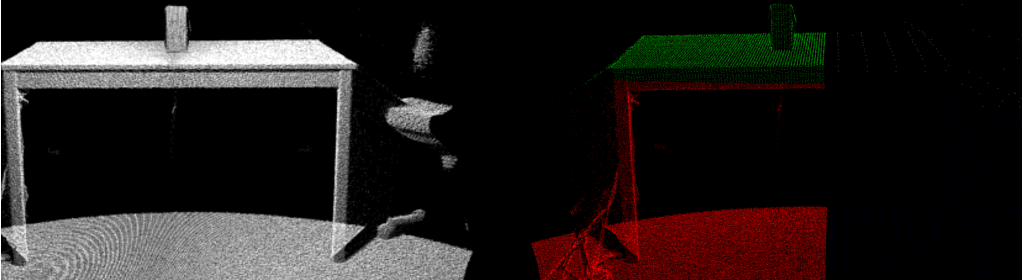
\includegraphics[width=1\textwidth]{images/lab1.png}
		\caption{\label{fig:lab1}Esempio di point cloud filtrata e colorata: a sinistra l'originale, a destra l'output.}
	\end{figure}


\section{Lab 2} \label{sec:lab2}

Descrizione bla bla

	\subsection{Algortimi utilizzati (teoria)}


	\subsection{Considerazioni}


\section{Lab 3} \label{sec:lab3}
Descrizione bla bla

	\subsection{Algortimi utilizzati (teoria)}

	\subsection{Considerazioni}


\section{Lab 4} \label{sec:lab4}
Descrizione bla bla

	\subsection{Algortimi utilizzati (teoria)}


	\subsection{Considerazioni}


\begin{thebibliography}{9}
\bibitem{nano3}
  K. Grove-Rasmussen og Jesper Nygård,
  \emph{Kvantefænomener i Nanosystemer}.
  Niels Bohr Institute \& Nano-Science Center, Københavns Universitet

\end{thebibliography}
\end{document}